%! TeX program = lualatex

% Gemini theme
% https://github.com/anishathalye/gemini

\documentclass[final]{beamer}

% ====================
% Packages
% ====================

\usepackage[T1]{fontenc}
\usepackage[francais]{babel}
\usepackage{lmodern}
\usepackage[size=a0,scale=1.18,orientation=portrait]{beamerposter}
\usetheme{gemini}
\usecolortheme{gemini}
\usepackage{graphicx}
\usepackage{booktabs}
\usepackage{multirow}
\usepackage{array}
\usepackage{tikz}
\usetikzlibrary{positioning}
\usepackage{pgfplots}
\pgfplotsset{compat=1.14}
\usepackage{anyfontsize}
\usepackage{graphbox}

% ====================
% Lengths
% ====================

% If you have N columns, choose \sepwidth and \colwidth such that
% (N+1)*\sepwidth + N*\colwidth = \paperwidth
\newlength{\sepwidth}
\newlength{\colwidth}
\setlength{\sepwidth}{0.025\paperwidth}
\setlength{\colwidth}{0.45\paperwidth}

\newcommand{\separatorcolumn}{\begin{column}{\sepwidth}\end{column}}

% ====================
% Title
% ====================

\title{TheoremView: A Framework for Extracting
Theorem-Like Environments from Raw PDFs}

\author{%
     \textbf{Shrey Mishra}
	 \and Neil Sharma
\and Antoine Gauquier
\and Pierre Senellart
}

\graphicspath{{img/}}

\institute[shortinst]{%
  \hfill
  
\includegraphics[height=3cm,align=c]{ens_psl} \hfill
  
\includegraphics[height=3cm,align=c]{cnrs} \hfill
  
\includegraphics[height=2cm,align=c]{inria} \hfill
  
\includegraphics[height=2.5cm,align=c]{iuf} \hfill
           \hfill\hfill
}

% ====================
% Footer (optional)
% ====================

\footercontent{
  \url{https://theoremkb.org/demo} \hfill
  \small European Conference on Information Retrieval (ECIR) 2025 --- Lucca, Italy \hfill
  \href{mailto:mishra_shrey@rocketmail.com}{\small mishra\_shrey@rocketmail.com} \hfill
  \textit{\small Video:} \url{https://theoremkb.org/video}
}
% (can be left out to remove footer)

% ====================
% Logo (optional)
% ====================

% use this to include logos on the left and/or right side of the header:
% \logoright{\includegraphics[height=7cm]{logo1.pdf}}
% \logoleft{\includegraphics[height=7cm]{logo2.pdf}}

% ====================
% Body
% ====================

\begin{document}

\begin{frame}[t]

	\begin{columns}[t]
		\begin{column}{.9\paperwidth}
			\centering
			\hspace{5em}
			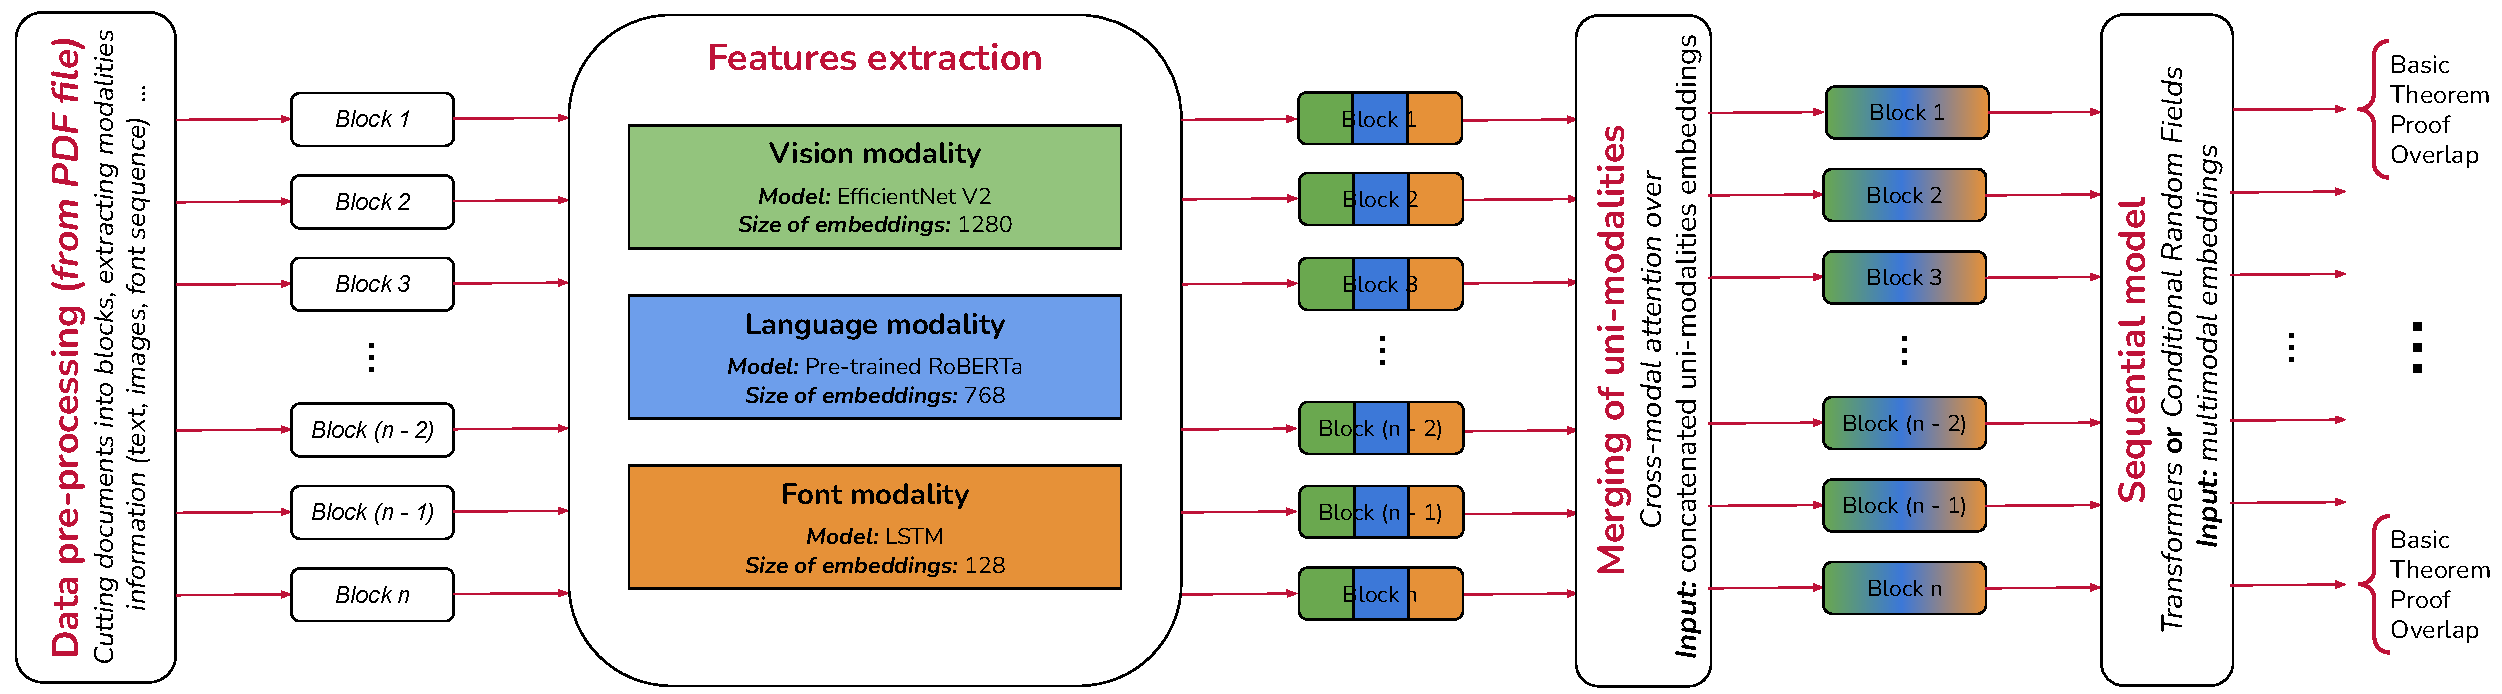
\includegraphics[width=0.8\linewidth]{img/general_pipeline}
			\hspace{5em}
		\end{column}
	\end{columns}

	\begin{columns}[t]
		\separatorcolumn

		\begin{column}{\colwidth}

			\begin{block}{System Architecture}
				The UI of the demo is organized into several segments:
				\begin{enumerate}
					\item \textbf{Upload and Process:} Users can upload PDFs or select from cached examples. The system processes PDFs using Grobid and pdfalto, converts pages to bitmap images, and merges XML outputs to generate a preprocessed data.csv file.
					\item \textbf{Predict and Preview:} Users can select unimodal or multimodal base models, with optional sequential processing using CRF, Transformer, or none, offering 12 possible combinations. Results can be previewed or downloaded (see Figure 4).
					\item \textbf{Summary and Statistics:} Provides a breakdown of inference time for current and cached runs, enabling comparative analysis.
				\end{enumerate}
				% 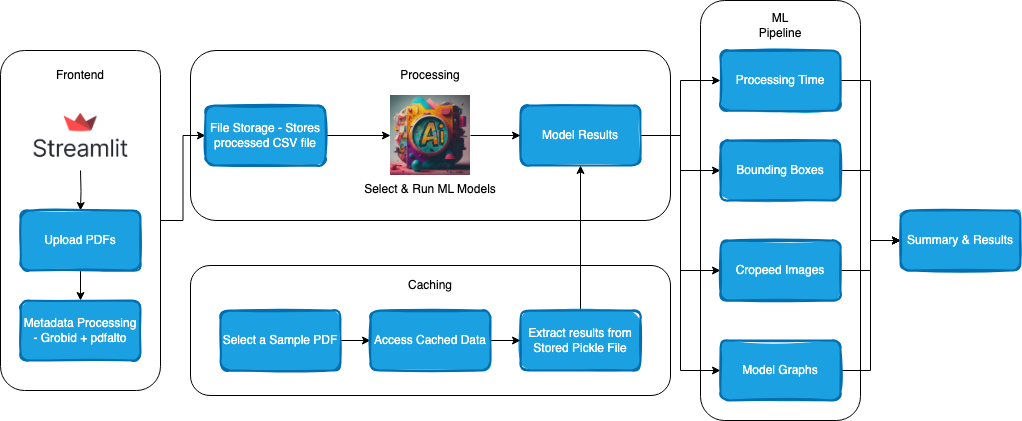
\includegraphics[width=0.9\linewidth]{img/sys-demo-arch.png}
			\end{block}

			\begin{block}{Model selection from the UI}
				\textbf{Base Models (as wide buttons):} One model is trained per modality:
				\begin{itemize}
					\item \textbf{Text.} A \textbf{RoBERTa} model is trained from scratch on a new corpus, consisting of the text from the paragraphs.
					\item \textbf{Vision.} Fine-tuning of \textbf{EfficientNet V2} on the bitmap rendering of the PDFs of the paragraphs.
					\item \textbf{Font Sequence.} A model \textbf{LSTM} is trained on the font sequences of each paragraph (a font token is given for each character of the paragraph).
					\item \textbf{Multimodal.} The cross-modal attention mechanism merges the three unimodalities, allowing for mapping interdependencies among different modalities.
				\end{itemize}

				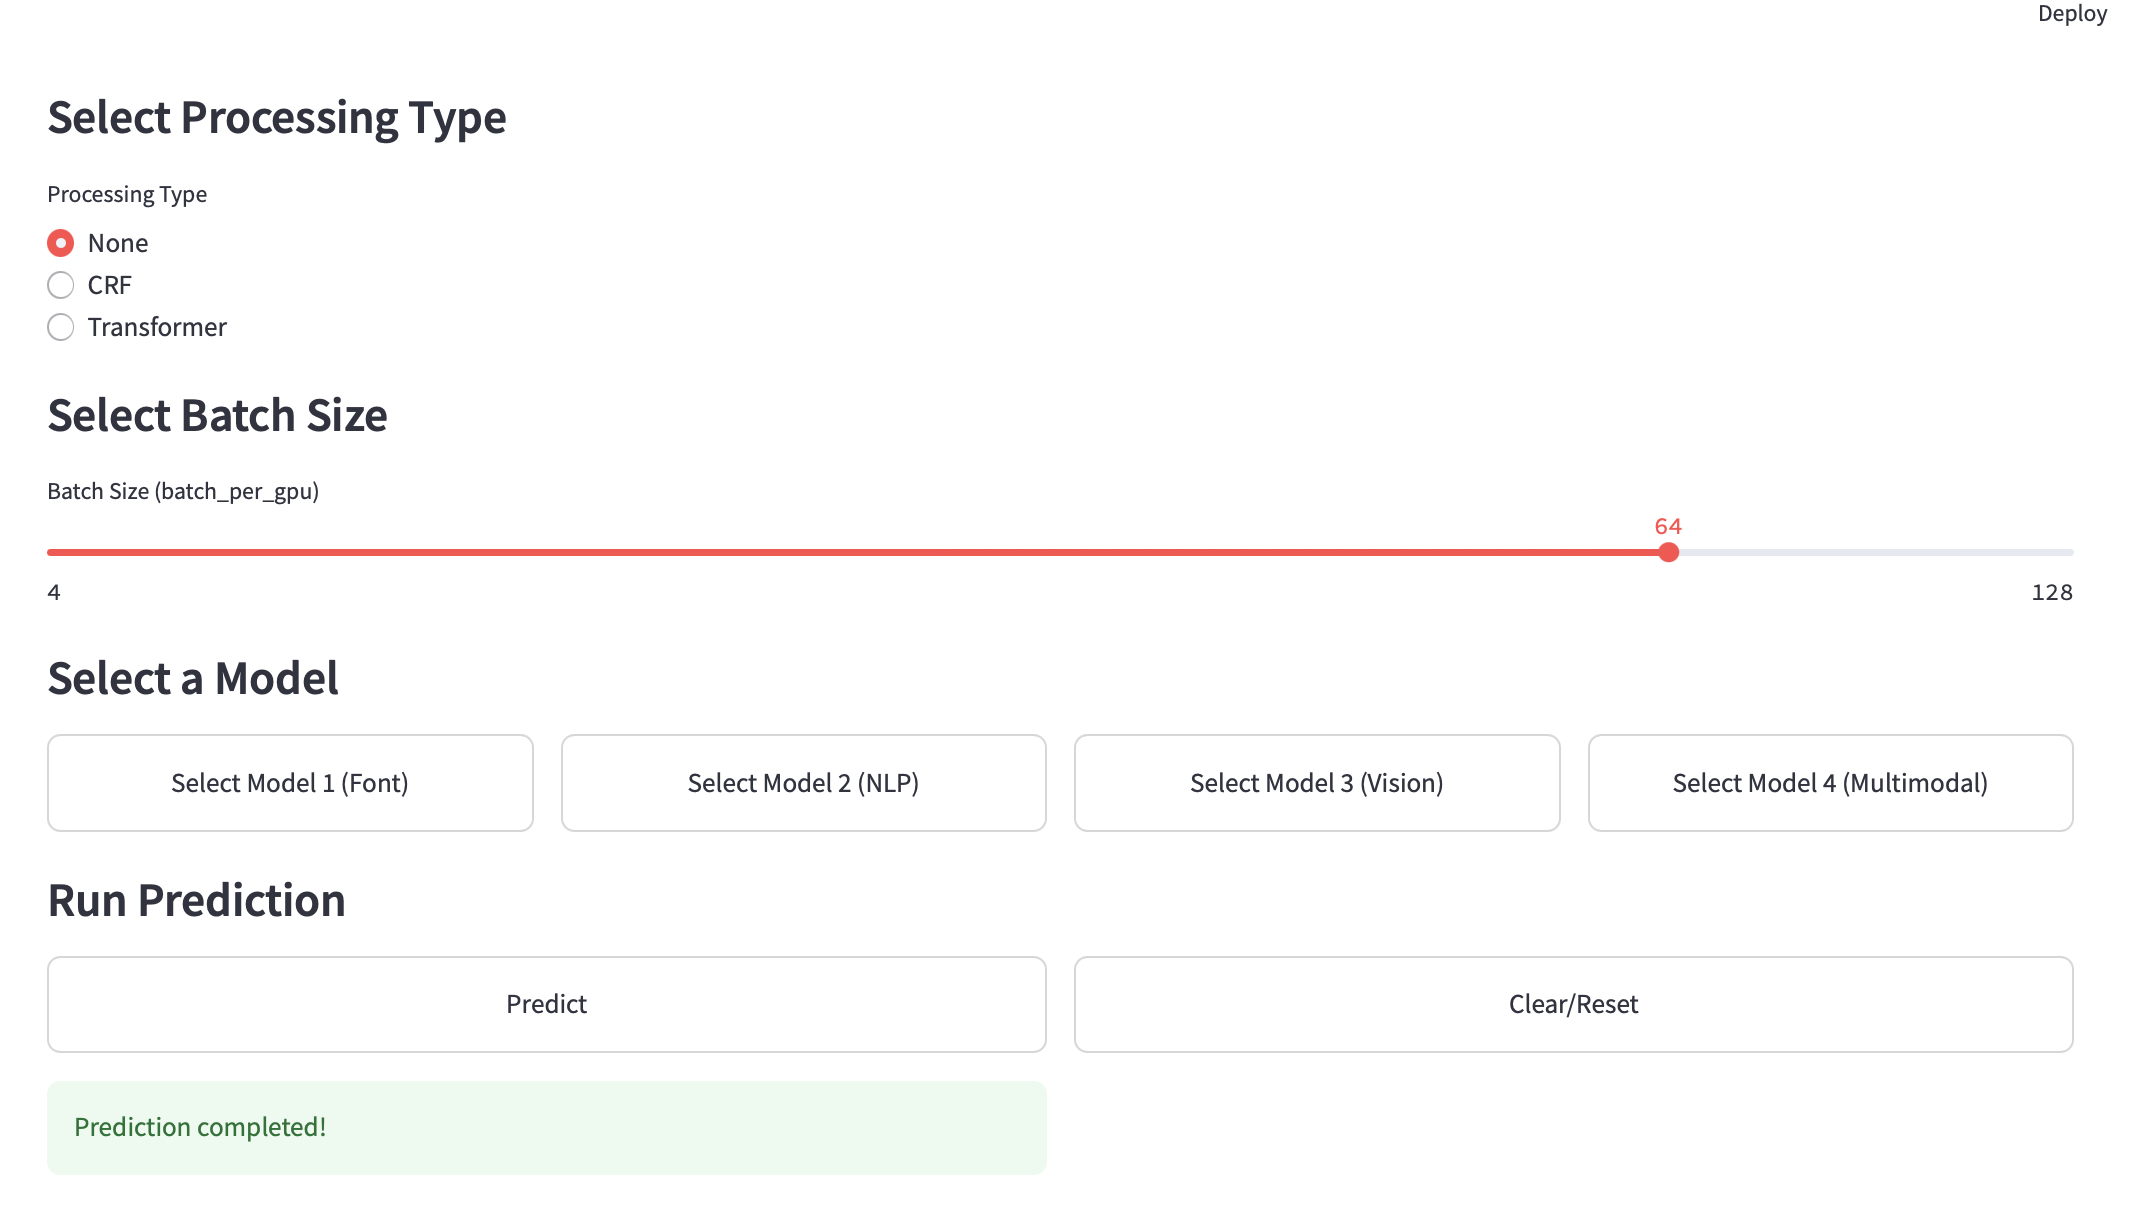
\includegraphics[width=\linewidth]{buttons.png}

				\textbf{Sequential Models (as radio buttons):} The order of paragraphs aids unimodal or multimodal models in classifying them correctly. Two tested architectures, a \textbf{Conditional Random Field (CRF)} and a \textbf{Transformer} with a sliding window, incorporate multimodal embeddings and sequence information. This includes the page number of each paragraph, its horizontal and vertical distances from the previous paragraph (based on bounding boxes), and a boolean indicating if it's on the same page as its predecessor. These features enhance the models' understanding of paragraph relationships.
				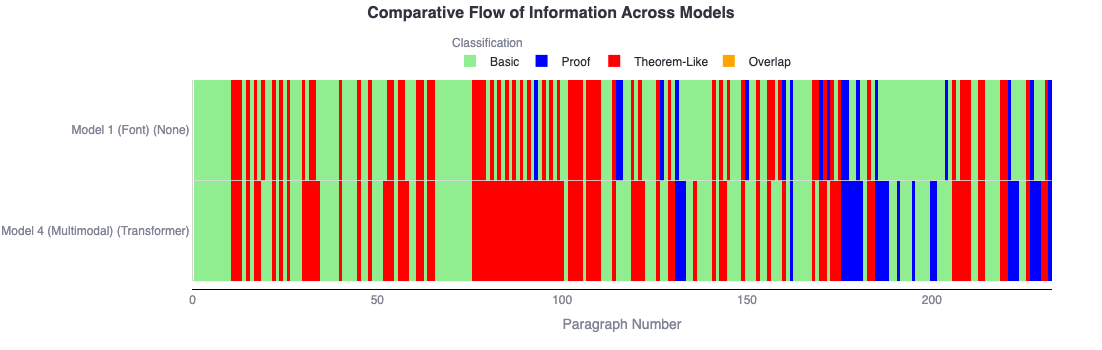
\includegraphics[width=\linewidth]{comparitive-v3.png}

			\end{block}

		\end{column}

		\separatorcolumn

		\begin{column}{\colwidth}

			\begin{block}{Data Preprocessing}
				Each PDF is pre-processed to extract different modalities. The source code \LaTeX{} is only necessary during the training phases to automatically generate annotated data. Only the PDF is required for inference.
				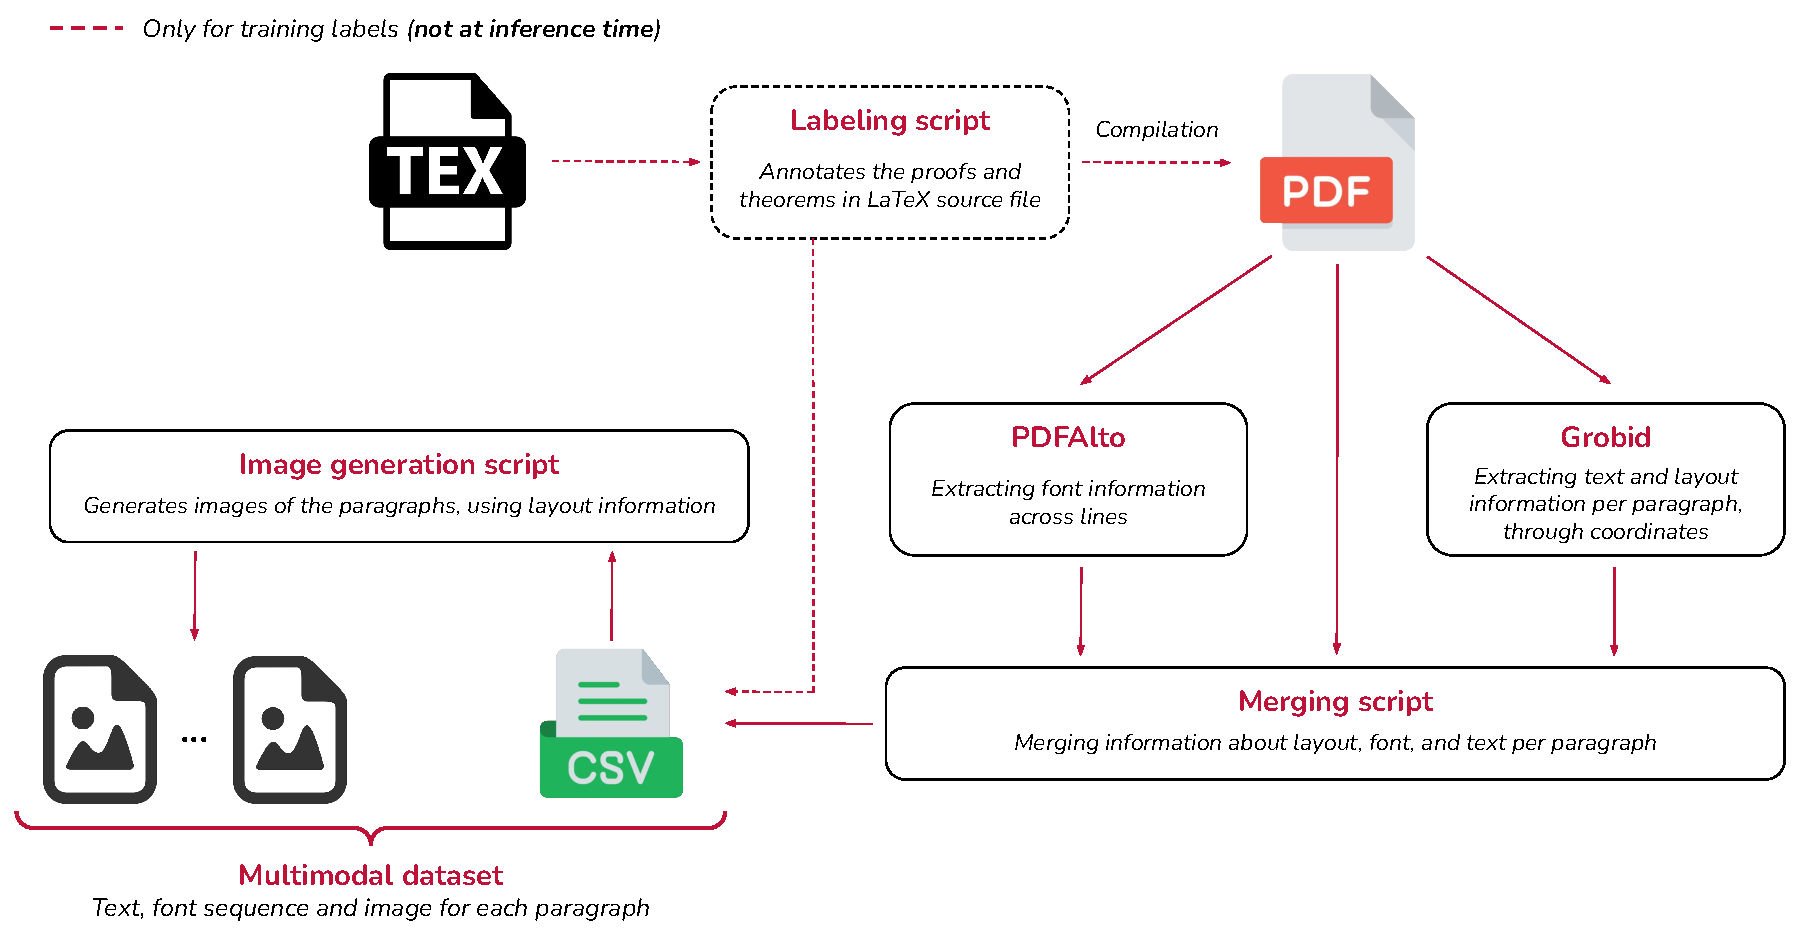
\includegraphics[width=\linewidth]{preprocessing}
			\end{block}

			\begin{block}{Results}
				Our model classifies paragraphs into four categories: \textbf{Proof}, \textbf{Theorem-like}, \textbf{Basic}, and an \textbf{Overlap reject class} due to preprocessing discrepancies. 
				
				\fbox{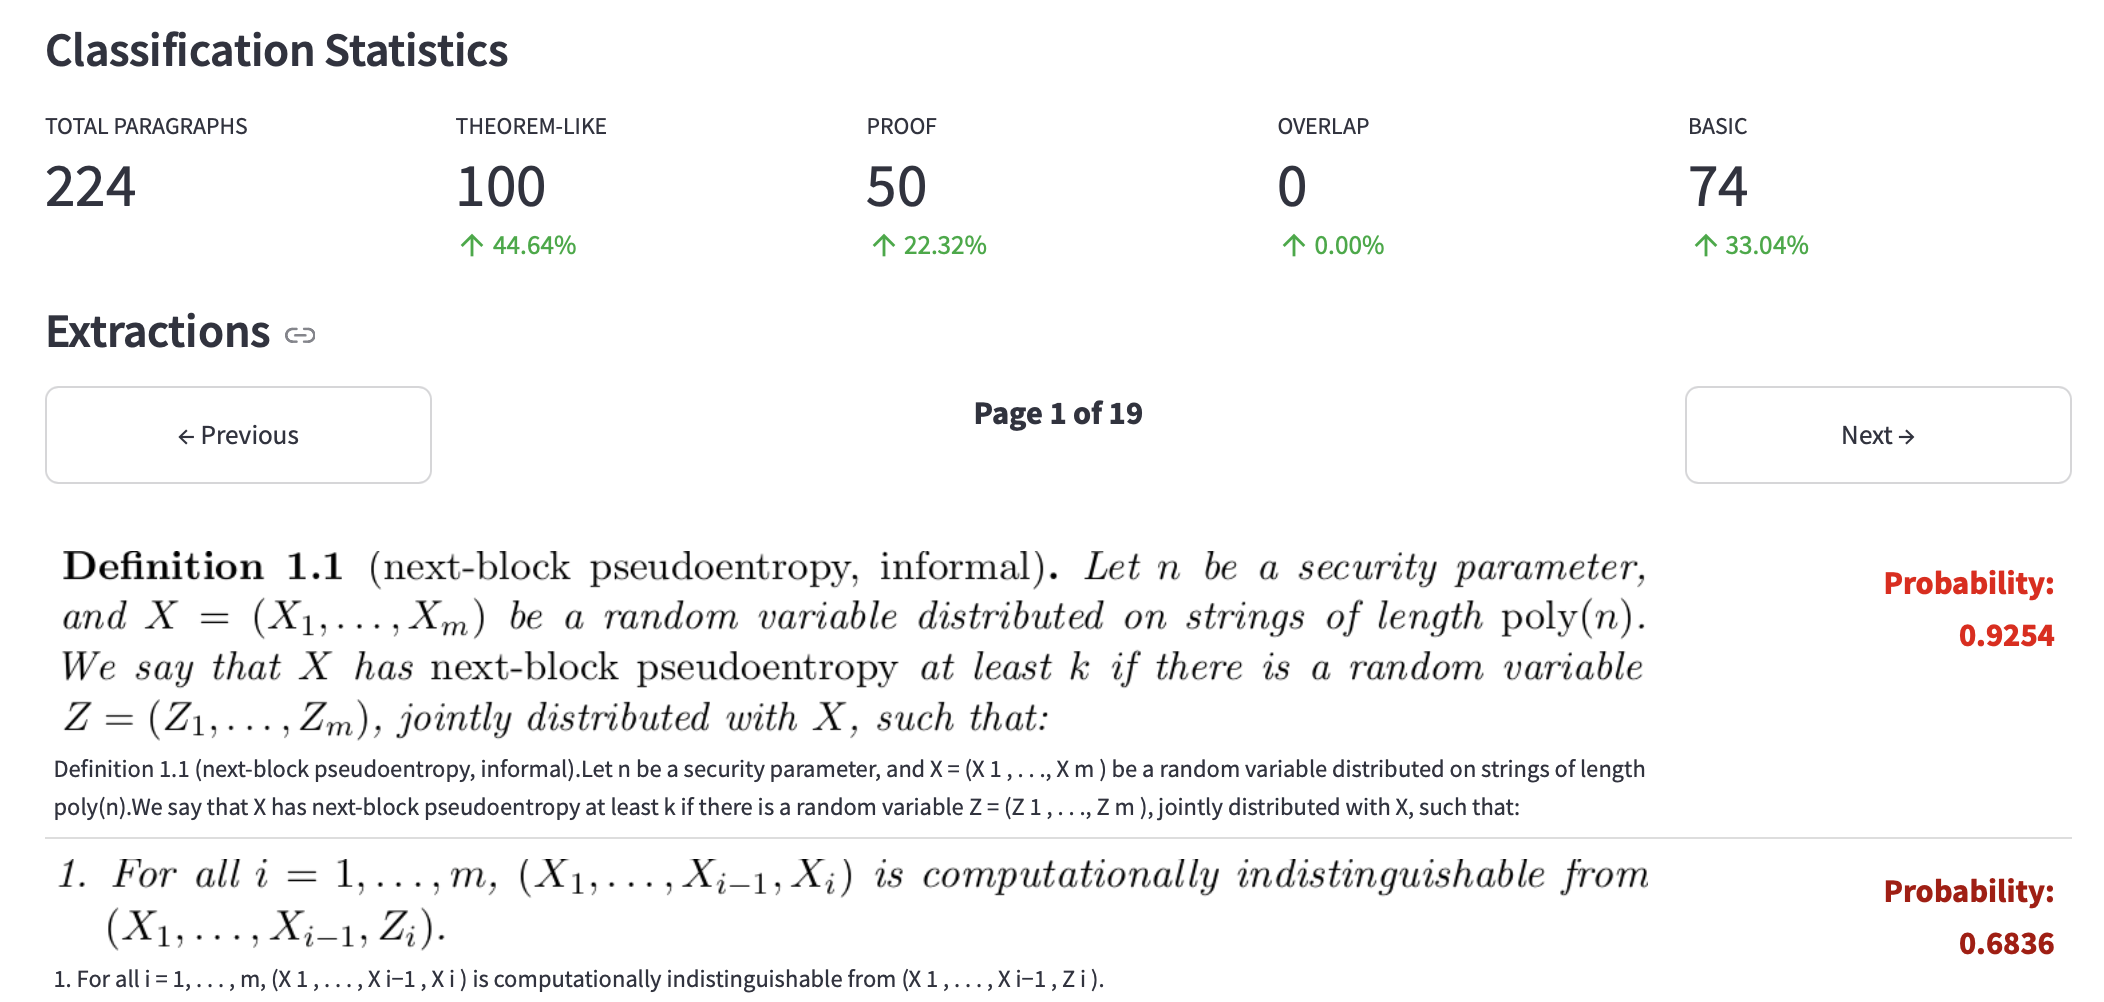
\includegraphics[width=\linewidth]{img/extractions.png}} % Updated to use 
				
				The \textbf{TheoremView demo interface}, built with Streamlit, features a modular design allowing users to upload PDFs or load from cached samples. It processes metadata with \textbf{Grobid} and \textbf{pdfalto}, storing results as CSV files. The pipeline supports prediction at various modalities with or without sequential information, generating processing times, bounding boxes, cropped theorem/proof images, and analytical graphs.

				\fbox{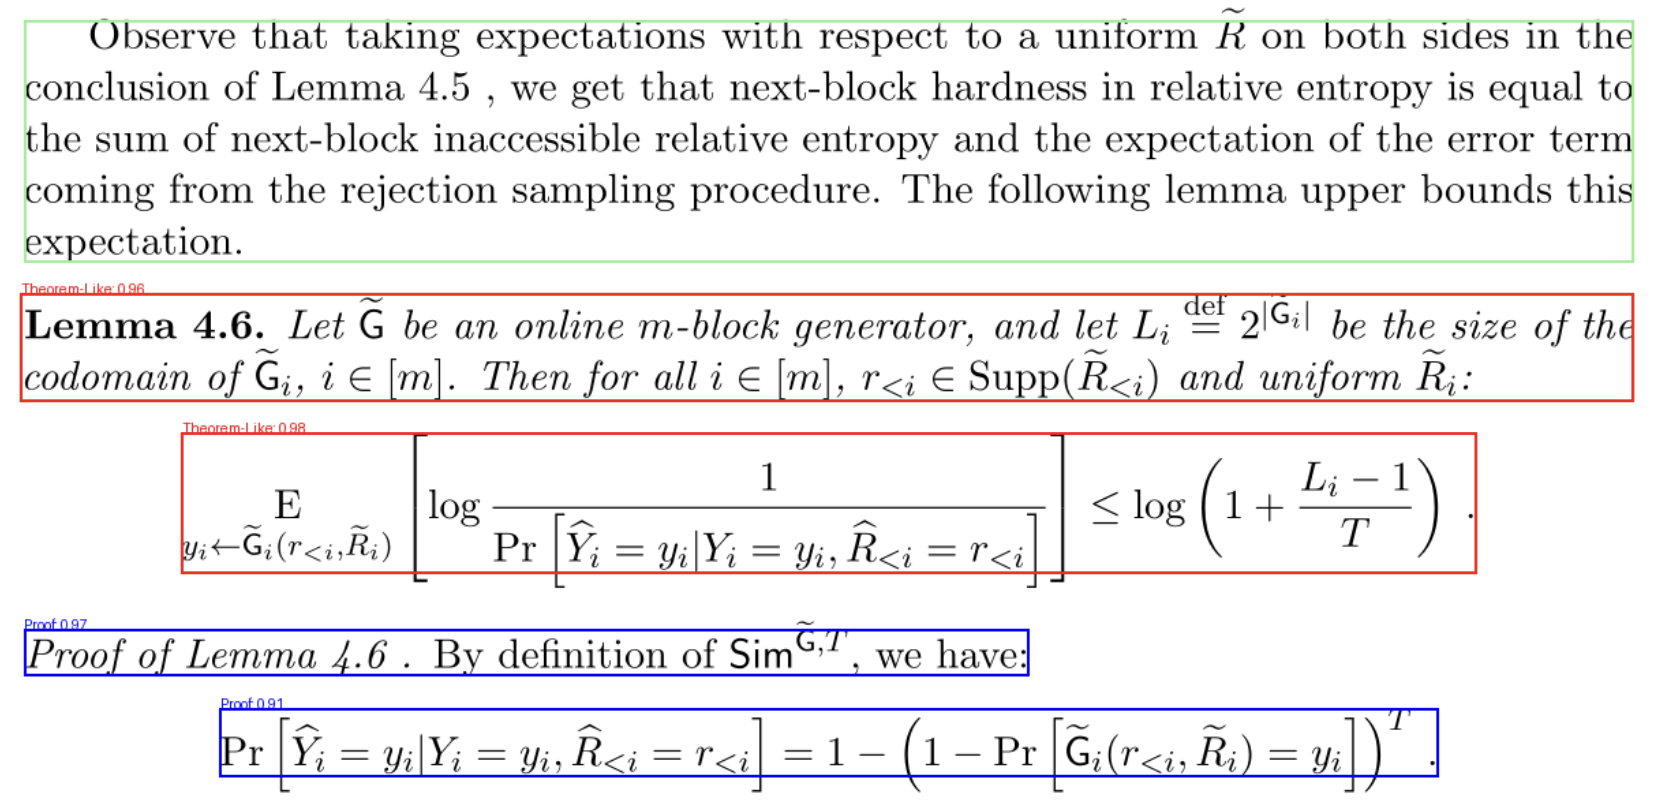
\includegraphics[width=\linewidth]{img/vis_on_pdf.png}} % Updated to use
				
				
				
				
				
				Efficient caching with \textbf{pickle files} enhances performance for frequently accessed data, ensuring scalability and precision in document analysis.
			\end{block}

			\vspace{-1.45em}

		\end{column}

		\separatorcolumn
	\end{columns}
\end{frame}

\end{document}
